\chapter{Project Management Methodology and Modeling}

\section{Introduction}
This chapter presents the project management methodology adopted by the Pengguin team for the development of Riaya. It focuses on the Kanban method, explaining its definition, fundamental principles, advantages, disadvantages, and a comparative analysis with other methodologies such as Scrum and Waterfall \cite{schwaber2020scrum, pmi2021pmbok}. It also justifies the choice of Kanban for this project. The second part of the chapter lists and presents the main modeling diagrams used to design the platform, including the use case diagram, class/ERD diagram, sequence diagram, activity diagram, deployment diagram, and the global BPMN model. Each diagram is accompanied by a detailed description of its purpose, its components, and its relevance to the Riaya project. The chapter aims to show how the combination of an agile methodology \cite{beck2001agile} and rigorous modeling practices allowed the Pengguin team to deliver a complex, AI-driven platform while maintaining quality, transparency, and adaptability.

\section{Presentation of the Kanban Method}

\subsection{Historical Context and Origins}
Kanban is an agile project management method that originated in the manufacturing industry, specifically at Toyota in Japan during the late 1940s, and was later adapted to software development and IT operations in the early 2000s \cite{anderson2010kanban}. The term ``Kanban'' means ``visual signal'' or ``card'' in Japanese. At Toyota, Kanban cards were used to signal the need for replenishment of parts on the production line, enabling a just-in-time (JIT) manufacturing system. The method was formalized for knowledge work by David J. Anderson in 2007, who introduced the concept of limiting Work in Progress (WIP) to improve flow in software teams \cite{anderson2010kanban}.

\subsection{Definition and Fundamental Principles}
The method is based on three fundamental principles that guide the daily work of the team: visualization, WIP limits, and flow management. These three principles form the backbone of Kanban and are complemented by a set of practices that help teams deliver value continuously.

\begin{itemize}
    \item \textbf{Visualization:} The workflow is represented on a board (physical or digital) divided into columns such as ``To Do'', ``In Progress'', ``Review'', and ``Done''. Each task is represented by a card that moves from left to right as work progresses. This visual representation allows all team members to see the status of the project at a glance, identify bottlenecks, and understand priorities without the need for lengthy meetings. In the Riaya project, visualization was essential because the work spanned multiple domains: frontend development, backend development, voice server integration, database design, DevOps, and quality assurance. Without a shared visual board, coordinating these activities would have been extremely difficult.

    \item \textbf{Work in Progress (WIP) Limits:} Each column has a maximum number of tasks that can be in progress simultaneously. This constraint helps identify bottlenecks and encourages the team to finish tasks before starting new ones. For example, if the ``In Progress'' column has a WIP limit of three, the team cannot start a fourth task until one of the three is completed or moved to another column. This practice reduces context switching, improves focus, and increases the overall throughput of the team \cite{anderson2010kanban}. In the Riaya project, WIP limits were particularly important during the integration of the OpenAI Realtime API, a complex task that required deep concentration and could not be interrupted by other work.

    \item \textbf{Flow Management:} The goal is to maintain a smooth and continuous flow of work. By limiting WIP, the team reduces context switching and improves cycle time. Flow management also involves measuring key metrics such as lead time (the time between task creation and completion) and cycle time (the time between task start and completion). These metrics help the team identify areas for improvement and optimize their workflow. In the Riaya project, the team tracked these metrics weekly and used them to adjust priorities and resource allocation.
\end{itemize}

\subsection{Kanban Practices and Metrics}
Beyond the three fundamental principles, Kanban relies on a set of practices that guide its implementation. These practices include making policies explicit, implementing feedback loops, and improving collaboratively. The most common Kanban metrics are:

\begin{itemize}
    \item \textbf{Lead Time:} The total time between the creation of a task and its completion.
    \item \textbf{Cycle Time:} The time between the start of work on a task and its completion.
    \item \textbf{Throughput:} The number of tasks completed per unit of time.
    \item \textbf{WIP:} The number of tasks currently in progress.
    \item \textbf{Flow Efficiency:} The ratio between value-adding time and total lead time.
\end{itemize}

In the Riaya project, these metrics were tracked using a digital board integrated with GitHub. Table~\ref{tab:kanban_metrics} summarizes the metrics and their interpretation in the project context.

\begin{table}[H]
    \centering
    \caption{Kanban Metrics Tracked in the Riaya Project}
    \label{tab:kanban_metrics}
    \small
    \begin{tabular}{p{3.5cm}p{5cm}p{4.5cm}}
        \toprule
        \textbf{Metric} & \textbf{Definition} & \textbf{Observation in Riaya} \\
        \midrule
        Lead time & Creation to completion & Average 5 days for a feature \\
        Cycle time & Start to completion & Average 2 days \\
        Throughput & Tasks completed per week & 8--12 tasks per week \\
        WIP & Tasks in progress & Limited to 3 per column \\
        Flow efficiency & Value-adding time ratio & Approximately 40\% \\
        \bottomrule
    \end{tabular}
    \\[0.2cm]
    \small Source: Author's own work based on Pengguin internal tracking.
\end{table}

\subsection{Kanban Board Used by the Pengguin Team}
In the context of the Riaya project, Kanban was implemented using a digital board (Trello, Jira, or a custom solution) that was accessible to all team members. The board included columns for ``Backlog'', ``To Do'', ``In Progress'', ``Code Review'', ``Testing'', and ``Done''. Each task was represented by a card containing a description, an assignee, a priority level, and an estimated effort. The team held short daily stand-up meetings to discuss progress, blockers, and priorities. The board was also integrated with GitHub, so that pull requests and commits were automatically linked to the corresponding cards, providing full traceability from requirements to code.

\begin{figure}[H]
    \centering
    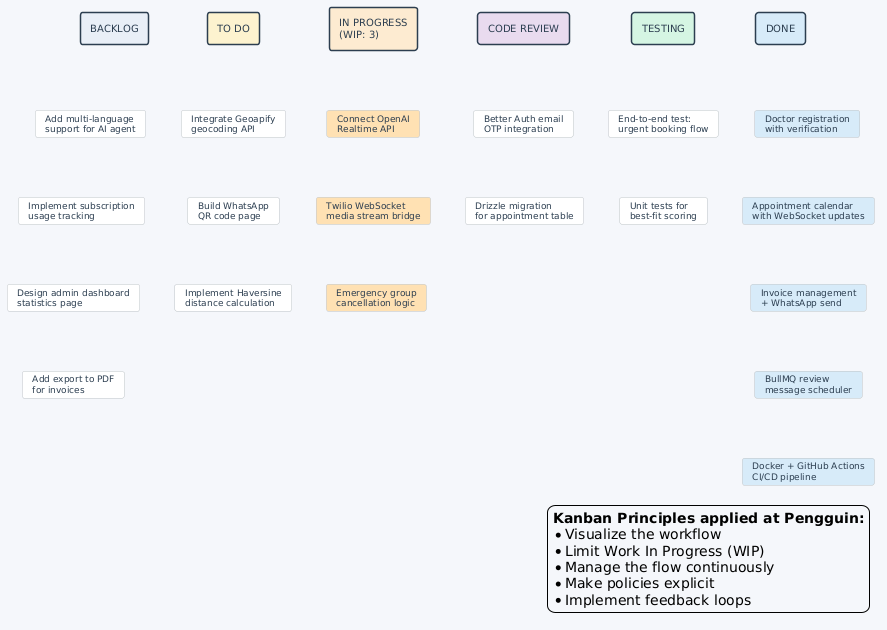
\includegraphics[width=0.8\textwidth]{images/kanban_board_example.png}
    \caption{Example of a Kanban Board Used by the Pengguin Team}
    \label{fig:kanban_board}
\end{figure}

Figure~\ref{fig:kanban_board} shows an example of the Kanban board used by the Pengguin team.

\subsection{Advantages of Kanban for the Riaya Project}
The Kanban method offers several advantages that are particularly relevant to the Riaya project:

\begin{itemize}
    \item \textbf{Flexibility:} Requirements can change at any time, which is essential when integrating AI and real-time communication features. In the Riaya project, the integration of the OpenAI Realtime API and Twilio required constant adjustments based on testing and client feedback \cite{twilio2024, openai2024realtime}. Kanban allowed the team to adapt quickly without being constrained by fixed sprint deadlines. For example, when the AI agent's language model needed to be fine-tuned to better understand Tunisian Arabic, the team was able to reprioritize tasks immediately without waiting for the next sprint.

    \item \textbf{Continuous Delivery:} Features can be delivered as soon as they are ready, allowing the client to provide feedback quickly. This was particularly valuable for the Riaya project, where the client wanted to see incremental progress and test features early. For example, the WhatsApp integration was delivered and tested before the AI voice agent was fully functional, allowing the client to validate the messaging workflow and provide feedback on the message templates.

    \item \textbf{Transparency:} The board gives all team members a clear view of the project status and priorities. This transparency reduces the need for status meetings and helps the team focus on the most important tasks. In the Riaya project, the board was accessible to both the development team and the project manager, ensuring that everyone had a shared understanding of the project's progress. The client also had read-only access to a simplified version of the board, which improved trust and communication.

    \item \textbf{Reduced Bottlenecks:} WIP limits help identify and resolve bottlenecks early, such as the integration of Twilio or OpenAI Realtime API. By limiting the number of tasks in progress, the team could focus on resolving blockers before they escalated. For example, when the Twilio integration encountered issues with WebSocket media streams, the team was able to dedicate resources to resolve the problem without being distracted by other tasks. This early detection prevented the bottleneck from delaying the entire project.

    \item \textbf{Improved Collaboration:} The visual nature of the board encourages communication and teamwork. Team members can see who is working on what and can offer help or advice when needed. In the Riaya project, the board facilitated collaboration between the frontend and backend developers, as well as between the web and voice server teams. When a frontend developer needed a new API endpoint, they could see which backend developer was working on the corresponding card and coordinate directly.

    \item \textbf{Metrics and Continuous Improvement:} Kanban encourages the collection and analysis of metrics such as lead time, cycle time, and throughput. These metrics help the team identify areas for improvement and make data-driven decisions. In the Riaya project, the team used these metrics to optimize their workflow and reduce the time required to deliver features. For example, after analyzing the cycle time of database migration tasks, the team decided to automate more of the migration process, reducing the average cycle time from three days to one day.
\end{itemize}

\subsection{Disadvantages and Limitations of the Method}
Despite its advantages, Kanban also has some limitations that the Pengguin team had to consider:

\begin{itemize}
    \item \textbf{Lack of Timeboxing:} Unlike Scrum, Kanban does not impose fixed iterations (sprints). This can lead to a lack of rhythm and deadlines if not managed carefully. In the Riaya project, the team mitigated this risk by setting internal deadlines and using time-based metrics to track progress. They also established a weekly review meeting to ensure that the project was moving forward at a satisfactory pace.

    \item \textbf{Role Ambiguity:} Kanban does not define specific roles such as Product Owner or Scrum Master. This can cause confusion in larger teams. In the Riaya project, the team was small and cross-functional, so role ambiguity was less of an issue. However, the project manager took on the responsibility of prioritizing tasks and ensuring that the board was up to date. Clear communication and regular stand-up meetings helped prevent misunderstandings.

    \item \textbf{Difficulty in Scaling:} For very large projects, Kanban can become difficult to coordinate without additional frameworks. In the Riaya project, the team was small enough to manage the board effectively. However, if the project were to grow, the team might need to adopt a scaling framework such as Scrum of Scrums or LeSS \cite{larman2016scaling}. This is an important consideration for future phases of the Riaya project.

    \item \textbf{Requires Discipline:} The team must be disciplined to respect WIP limits and keep the board updated. In the Riaya project, the team held daily stand-up meetings to ensure that the board was accurate and that WIP limits were respected. Without this discipline, the board could become outdated and lose its value. The project manager also performed regular audits of the board to ensure that it reflected reality.

    \item \textbf{Lack of Emphasis on Quality:} Kanban does not prescribe specific quality practices such as test-driven development (TDD) or code reviews \cite{beck2002tdd}. In the Riaya project, the team adopted these practices independently to ensure the quality of the code. The ``Code Review'' and ``Testing'' columns on the board helped enforce these practices. Automated tests were run on every pull request, and code reviews were mandatory before merging.
\end{itemize}

\subsection{Comparative Table: Kanban vs Scrum vs Waterfall (V-Model)}
Table~\ref{tab:comparison_methods} compares the three main project management methodologies considered by the Pengguin team.

\begin{table}[H]
    \centering
    \caption{Comparison of Kanban, Scrum, and Waterfall}
    \label{tab:comparison_methods}
    \small
    \begin{tabular}{p{2.5cm}p{3.5cm}p{3.5cm}p{3.5cm}}
        \toprule
        \textbf{Criteria} & \textbf{Kanban} & \textbf{Scrum} & \textbf{Waterfall (V-Model)} \\
        \midrule
        Approach & Continuous flow & Iterative (sprints) & Sequential \\
        Roles & Not defined & Product Owner, Scrum Master, Team & Project Manager \\
        Changes & At any time & Between sprints & Difficult after validation \\
        Delivery & Continuous & At the end of each sprint & At the end of the project \\
        WIP Limits & Yes & Implicit (sprint backlog) & No \\
        Meetings & Daily stand-up (optional) & Sprint planning, daily stand-up, review, retrospective & Milestone reviews \\
        Metrics & Lead time, cycle time, throughput & Velocity, burndown chart & Earned value management \\
        Best suited for & Support, DevOps, evolving projects & Complex products with changing requirements & Projects with fixed requirements \\
        \bottomrule
    \end{tabular}
    \\[0.2cm]
    \small Source: Adapted from Kniberg, H., \& Skarin, M. (2010). \textit{Kanban and Scrum: Making the Most of Both}. InfoQ \cite{kniberg2010kanban}.
\end{table}

\subsection{Justification of the Choice of Kanban by the Pengguin Team}
The Pengguin team chose Kanban for the Riaya project for several reasons.

First, the project involves a high degree of uncertainty and innovation, particularly in the integration of AI voice agents and real-time WebSocket communication. Kanban's flexibility allows the team to adapt quickly to technical challenges and client feedback. When the OpenAI Realtime API was first integrated, its behaviour differed from initial assumptions, and the team needed to adjust the prompt engineering and tool calling strategy. Kanban allowed this without disrupting the overall schedule.

Second, the project is developed by a small, cross-functional team that can benefit from the transparency and self-organization promoted by Kanban. Each developer was responsible for multiple areas (frontend, backend, DevOps), and the board helped them coordinate without the overhead of formal ceremonies.

Third, the continuous delivery model aligns well with the client's desire to see incremental progress and to test features early. The client was able to test the WhatsApp integration, the AI voice agent, and the doctor dashboard at different stages, providing valuable feedback that shaped subsequent iterations.

Fourth, the use of a digital Kanban board facilitates remote collaboration and integration with the CI/CD pipeline. The board was accessible from any device, and the GitHub integration ensured that each pull request was linked to its corresponding card. This provided full traceability from requirements to code and helped the team maintain a clear overview of the project at all times.

Finally, an important factor in the choice of Kanban was the need to handle urgent production issues alongside planned development work. Because Riaya is a live platform that handles real patient calls, the team needed a method that could accommodate unplanned work without disrupting the entire schedule. Kanban's flexible structure allowed the team to insert urgent tasks into the board and to prioritize them without having to wait for the next sprint. This was particularly valuable during the early weeks of production, when unexpected issues required immediate attention.

\begin{figure}[H]
    \centering
    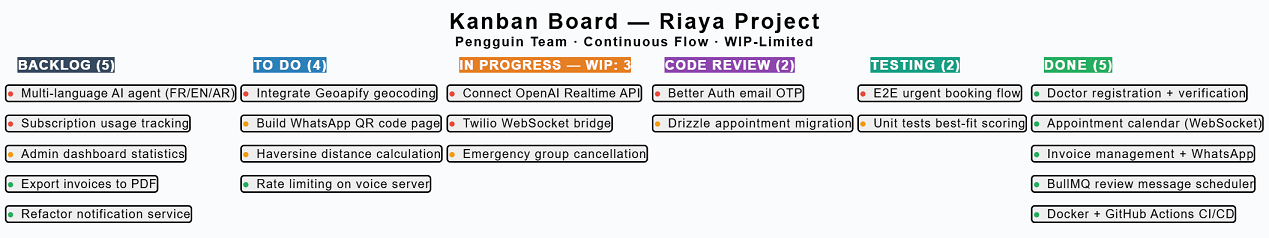
\includegraphics[width=0.8\textwidth]{images/kanban_board_riaya.png}
    \caption{Kanban Board Used in the Riaya Project}
    \label{fig:kanban_riaya}
    \small Source: Pengguin Internal Documentation.
\end{figure}

Figure~\ref{fig:kanban_riaya} shows the Kanban board actually used during the Riaya project.

\section{List and Presentation of Modeling Diagrams}
The modeling of a complex system such as Riaya requires a set of complementary diagrams, each capturing a different view of the system \cite{omg2017uml, fowler2003uml}. The Pengguin team used six main diagrams: the use case diagram, the class/ERD diagram, the sequence diagram, the activity diagram, the deployment diagram, and the BPMN diagram. The following subsections present each of them in detail.

\subsection{Use Case Diagram: Presentation of Actors and Their Interactions}
The use case diagram provides a high-level view of the interactions between the actors (Patient, Doctor, Administrator) and the Riaya system. It shows the main use cases such as ``Book an appointment'', ``Manage patients'', ``Verify doctors'', and ``Monitor live calls''. This diagram is essential for understanding the functional scope of the platform and for communicating with stakeholders who may not be familiar with technical details.

The use case diagram includes three main actors:

\begin{itemize}
    \item \textbf{Patient:} The patient interacts with the system through phone calls and WhatsApp. The main use cases include ``Call Riaya and speak with the booking assistant'', ``Book an appointment'', ``Request urgent booking'', ``Consult or cancel an existing AI booking'', ``Receive doctor messages on WhatsApp'', ``Rate a doctor after a visit'', and ``Be notified if a request expires''. The patient does not need to authenticate because the phone number is used as the unique identifier.
    
    \item \textbf{Doctor:} The doctor interacts with the system through a web dashboard. The main use cases include ``Register and apply for verification'', ``Manage practice profile and availability'', ``Manage patients'', ``Manage appointments'', ``Manage medical documentation'', ``Manage patient billing'', ``Record and transcribe consultations'', ``Use the practice AI assistant'', ``Connect WhatsApp'', and ``Manage Riaya subscription''. Most of these use cases require the doctor to be authenticated and verified.
    
    \item \textbf{Administrator:} The administrator interacts with the system through a dedicated back-office. The main use cases include ``Review and verify doctors'', ``Monitor the AI booking channel'', ``Operate platform configuration'', and ``View platform overview''. The administrator has the highest level of access and can manage all aspects of the platform.
\end{itemize}

The use case diagram also shows the relationships between use cases, such as ``include'' and ``extend''. For example, the ``Book an appointment'' use case includes ``Authenticate'' for the doctor, and the ``Register and apply for verification'' use case includes ``Verify email OTP''. These relationships help clarify the dependencies between use cases and ensure that all necessary steps are accounted for.

\begin{figure}[H]
    \centering
    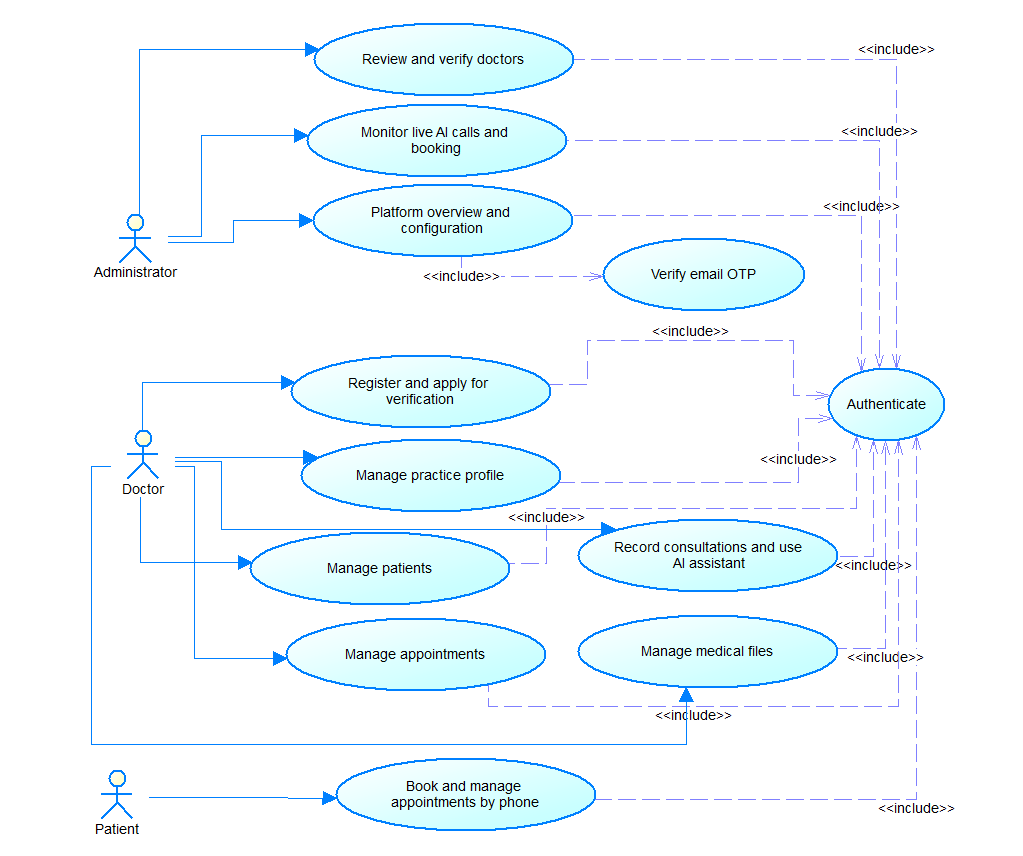
\includegraphics[width=0.8\textwidth]{images/use_case_diagramdsdsd.png}
    \caption{Use Case Diagram of Riaya}
    \label{fig:use_case}
\end{figure}

The use case diagram presented in Figure~\ref{fig:use_case} provides a high-level view of the interactions between the three main actors of the Riaya platform --- the Patient, the Doctor, and the Administrator --- and the system itself. The system boundary is represented by the rectangle labelled ``Riaya'', which encloses all the use cases offered by the platform.

The \textbf{Patient} interacts with the system exclusively through phone calls and WhatsApp, without any account creation. The patient's use cases include: \textit{Call Riaya and speak with the AI assistant}, \textit{Book an appointment (standard or urgent)}, \textit{Consult or cancel pending appointments}, \textit{Receive WhatsApp messages from the doctor}, \textit{Rate a doctor after a visit}, and \textit{Be notified if a request expires}.

The \textbf{Doctor} interacts with the system through a secure web dashboard. The doctor's use cases include: \textit{Register and apply for verification}, \textit{Manage practice profile and availability}, \textit{Manage patients}, \textit{Manage appointments}, \textit{Manage medical files and documents}, \textit{Manage invoices and send via WhatsApp}, \textit{Record consultations and use the AI assistant}, and \textit{Manage subscription and connect WhatsApp}. Most of these use cases require the doctor to be authenticated and verified.

The \textbf{Administrator} uses a dedicated back-office. The administrator's use cases include: \textit{Review and verify doctors}, \textit{Monitor live AI calls and booking}, and \textit{Platform overview and configuration}.

The diagram also shows the \texttt{<<include>>} relationships. For example, the \textit{Register and apply for verification} use case includes \textit{Verify email OTP}, which is a mandatory step. Similarly, all doctor and administrator use cases that require dashboard access include the \textit{Authenticate (sign in)} use case. These relationships clarify the dependencies between use cases and ensure that all necessary steps are accounted for in the functional design of the platform.

Overall, the use case diagram helps to communicate the functional scope of Riaya to both technical and non-technical stakeholders, and it serves as a reference for validating that all user needs are covered by the system.

\subsection{Class Diagram / ERD: Modeling the PostgreSQL Database}
The class diagram, also known as the Entity-Relationship Diagram (ERD), models the database schema of the Riaya platform. It includes entities such as \texttt{doctor\_profile}, \texttt{patient}, \texttt{appointment}, \texttt{invoice}, \texttt{consultation}, \texttt{whatsapp\_session}, and \texttt{subscription}. The ERD shows the relationships between these entities, including cardinalities (one-to-many, many-to-one) and key attributes. This diagram is crucial for designing the PostgreSQL database \cite{postgresql2024} accessed through Drizzle ORM \cite{drizzle2024}.

The main entities and their relationships are as follows:

\begin{itemize}
    \item \textbf{Doctor\_Profile:} Stores the professional information of the doctor, including first name, last name, CIN picture, speciality, Medical Council registration number, Medical Council certificate, cabinet name, TIN, cabinet city, and exact cabinet location (latitude and longitude). A doctor has one profile and can have many appointments, consultations, invoices, and WhatsApp sessions.
    
    \item \textbf{Patient:} Stores the patient's information, including first name, last name, date of birth, gender, address, preferred language, and phone number. A patient can have many appointments and consultations. The phone number is the unique identifier and is used to match the caller when they dial the Riaya number.
    
    \item \textbf{Appointment:} Stores the appointment details, including date and time, status (pending, confirmed, cancelled), reason for the visit, and emergency group ID (for urgent requests). An appointment is linked to one doctor and one patient. The emergency group ID allows multiple urgent appointments to be linked together so that they can be cancelled as a group if needed.
    
    \item \textbf{Invoice:} Stores the invoice details, including amount, status (paid, unpaid), and date. An invoice is linked to one doctor and one patient. Invoices can be sent to the patient via WhatsApp.
    
    \item \textbf{Consultation:} Stores the consultation notes, prescriptions, and medical documents. A consultation is linked to one doctor and one patient. Medical documents are stored in Cloudflare R2 \cite{cloudflare2024r2}, and the consultation record contains a reference to the stored file.
    
    \item \textbf{WhatsApp\_Session:} Stores the WhatsApp session details, including the linked phone number and session status. A WhatsApp session is linked to one doctor. The session is established when the doctor scans a QR code, and it allows the platform to send messages from the doctor's own number.
    
    \item \textbf{Subscription:} Stores the subscription details, including plan type (Free or Pro), start date, end date, and usage limits. A subscription is linked to one doctor. Usage limits are tracked to enforce the Free plan restrictions.
\end{itemize}

The ERD also includes join tables and foreign keys that enforce referential integrity. For example, the \texttt{appointment} table has foreign keys pointing to both the \texttt{doctor\_profile} and \texttt{patient} tables, ensuring that every appointment is associated with a valid doctor and patient. The use of Drizzle ORM allows these relationships to be defined in TypeScript, providing type safety and reducing the risk of runtime errors.

\begin{figure}[H]
    \centering
    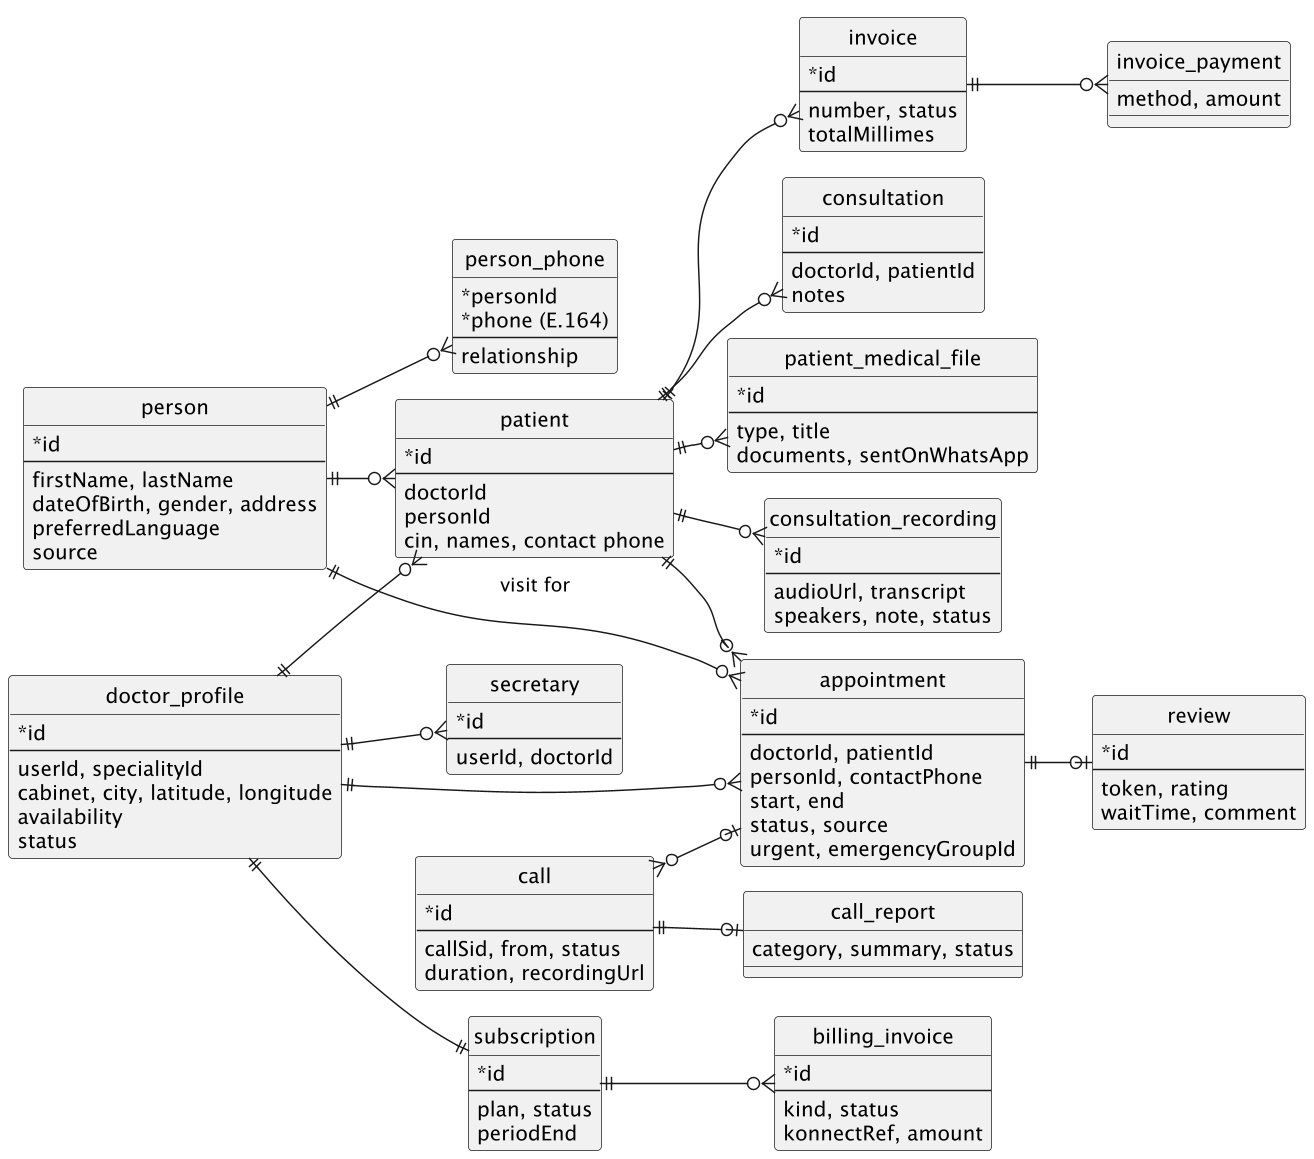
\includegraphics[width=0.9\textwidth]{images/erd_diagram.png}
    \caption{Entity-Relationship Diagram of the Riaya Database}
    \label{fig:erd}
\end{figure}

Figure~\ref{fig:erd} presents the complete ERD of the Riaya database, showing all entities and their relationships.

\subsection{Sequence Diagram: Twilio Call Flow \texorpdfstring{$\rightarrow$}{→} WebSocket \texorpdfstring{$\rightarrow$}{→} OpenAI \texorpdfstring{$\rightarrow$}{→} Database}
The sequence diagram illustrates the real-time flow of a patient's phone call. It shows the interactions between Twilio, the Express.js voice server, the OpenAI Realtime API (via Microsoft Azure), and the PostgreSQL database. The diagram details how the call is received, how the WebSocket media stream is established, how the AI processes speech and makes tool calls to the database, and how the live transcript is sent to the admin dashboard.

The sequence of events is as follows:

\begin{enumerate}
    \item The patient dials the Riaya phone number.
    \item Twilio receives the call and sends a webhook to the Express.js voice server.
    \item The Express.js server looks up or creates the caller in the PostgreSQL database. If the caller is new, a patient record is created with the phone number as the unique identifier.
    \item The server responds with TwiML that opens a WebSocket media stream from Twilio to the server.
    \item The server establishes a WebSocket connection with the OpenAI Realtime API (via Microsoft Azure).
    \item The patient's speech is streamed to the AI, and the AI's voice is streamed back through Twilio onto the phone.
    \item The AI makes tool calls to the database to search for doctors, check availability, and create appointments. These tool calls are executed by the Express.js server, which queries the database and returns the results to the AI.
    \item The live transcript is sent to the admin dashboard via WebSocket, allowing administrators to monitor the call in real time.
    \item When the call ends, the Twilio stream closes, and the session is marked as completed in the database.
\end{enumerate}

This sequence diagram is particularly important because it captures the complexity of the real-time interaction between multiple systems. It helps developers understand the flow of data and the responsibilities of each component, and it serves as a reference for debugging and optimization.

\begin{figure}[H]
    \centering
    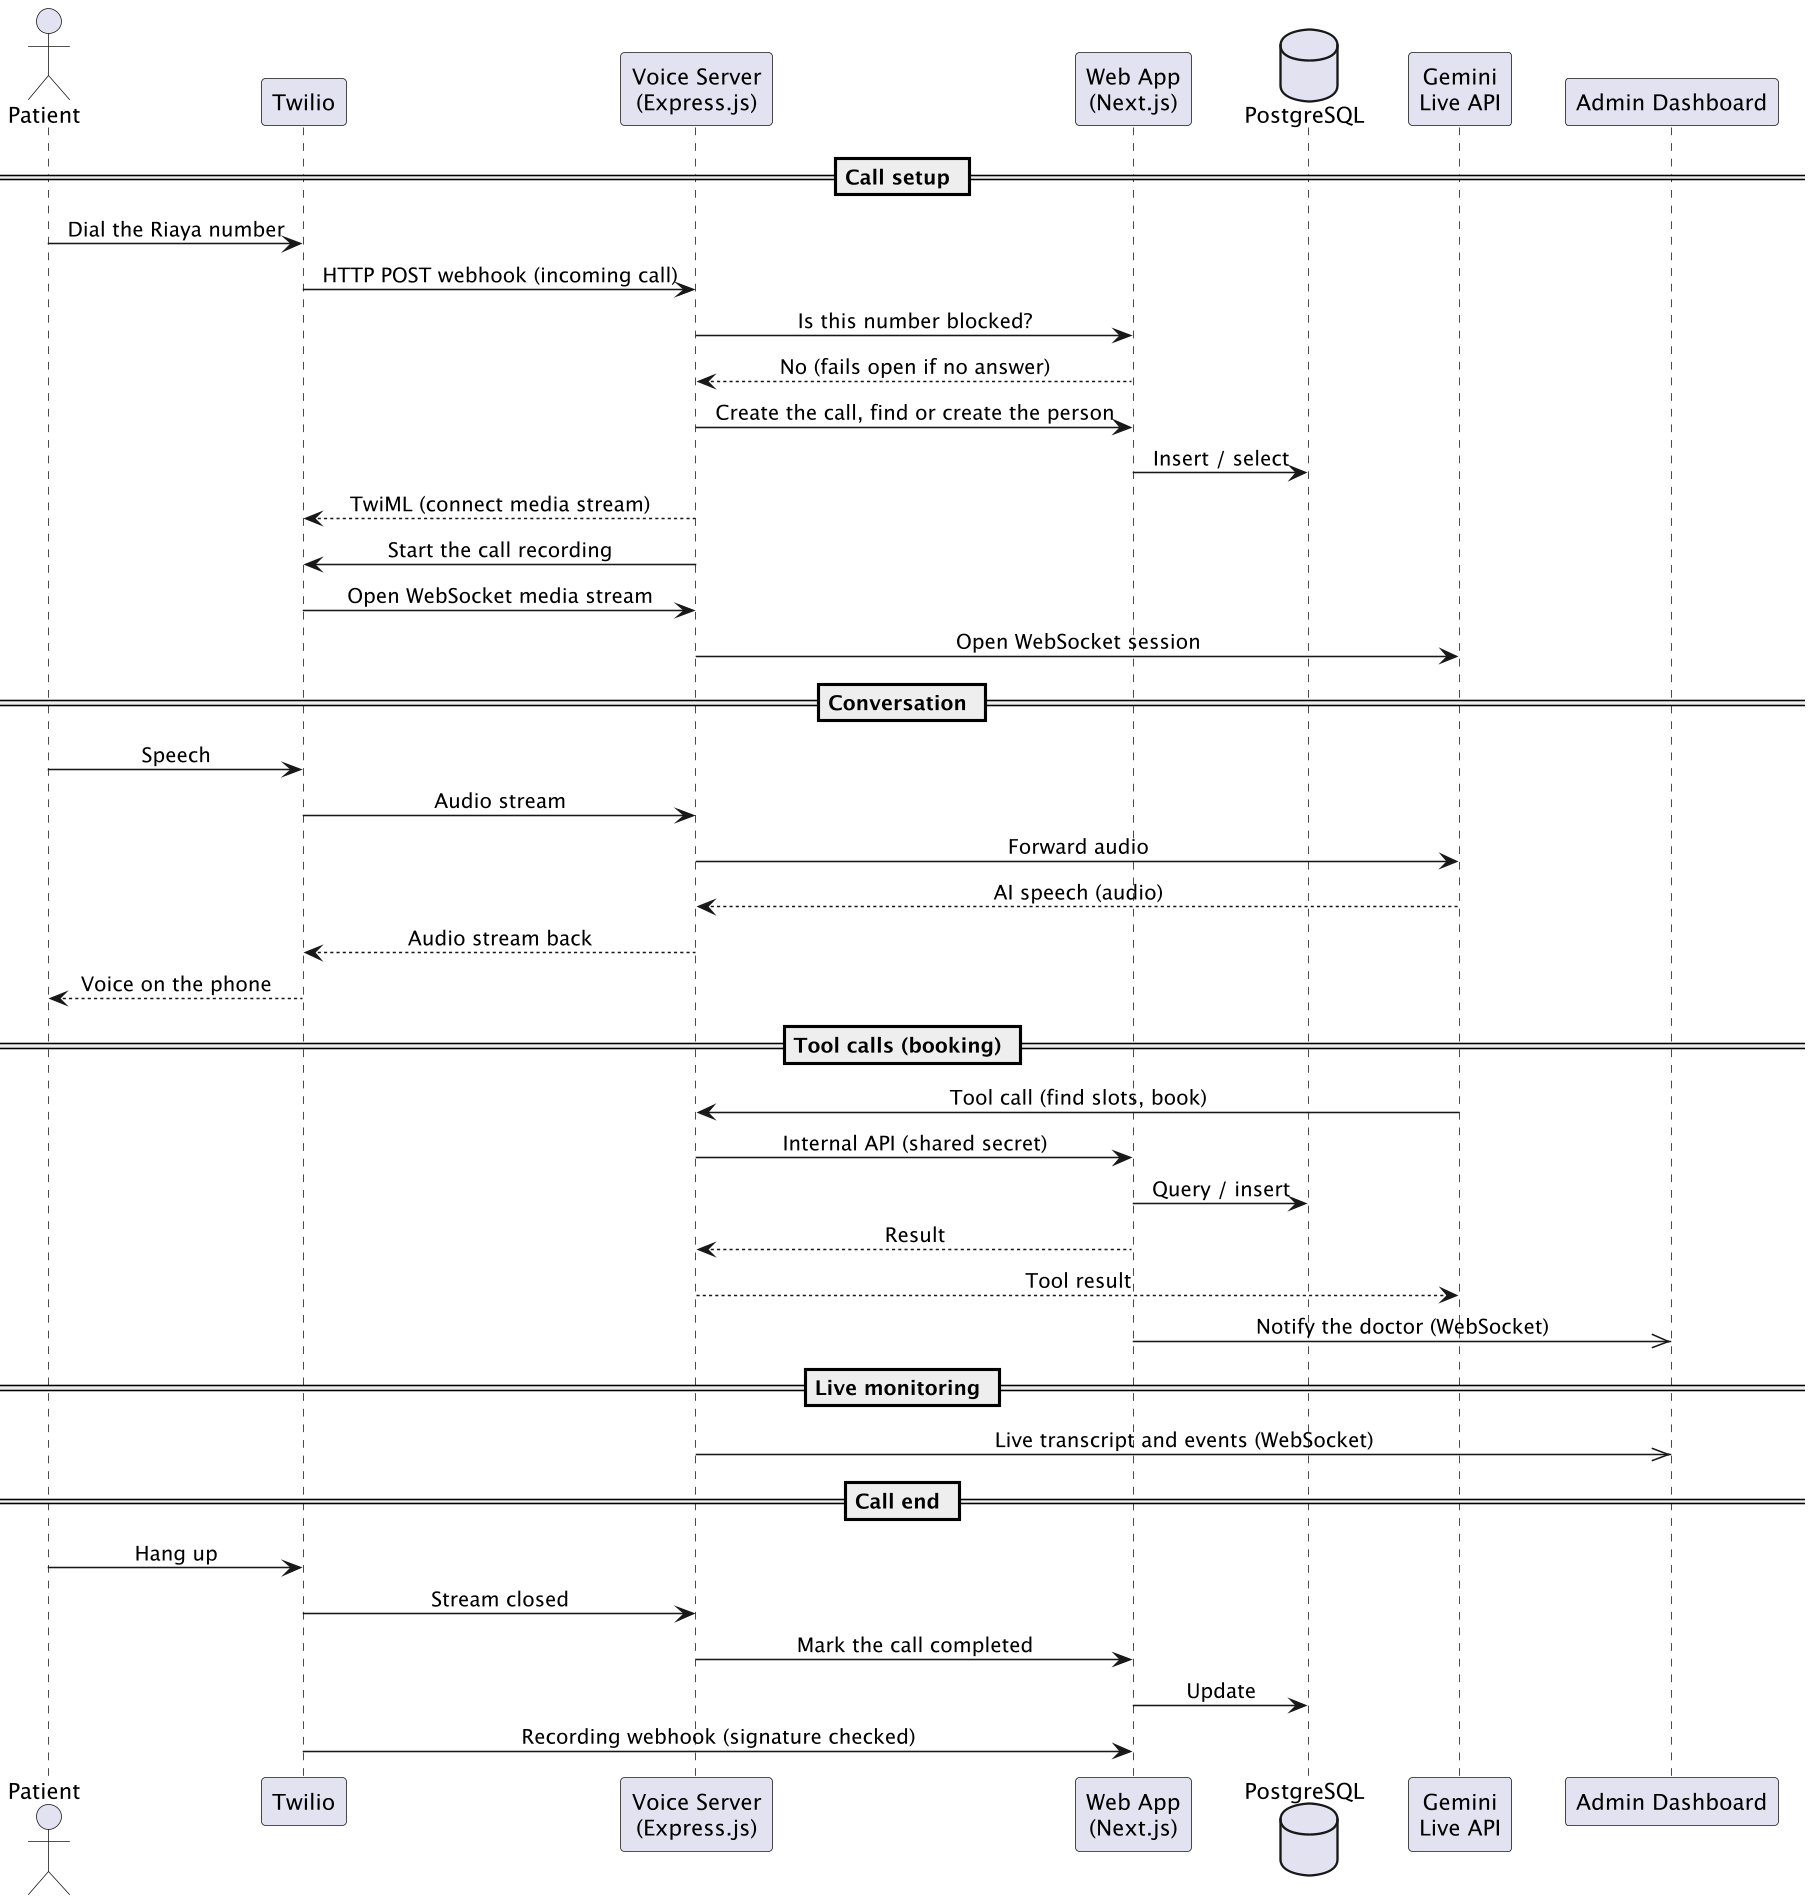
\includegraphics[width=0.9\textwidth]{images/sequence_call_flow.png}
    \caption{Sequence Diagram of the AI Call Flow}
    \label{fig:sequence_call}
\end{figure}

The sequence diagram presented in Figure~\ref{fig:sequence_call} illustrates the real-time flow of a patient's phone call through the Riaya platform. It captures the interactions between six main components: the Patient, Twilio (telephony provider), the Express.js Voice Server, the OpenAI Realtime API (accessed via Microsoft Azure), the PostgreSQL database (managed through Drizzle ORM), and the Admin Dashboard. This diagram is particularly important because it highlights the complexity of the real-time interaction between multiple systems and clarifies the responsibilities of each component.

The sequence begins when the \textbf{Patient} dials the Riaya phone number. \textbf{Twilio} receives the call and sends an HTTP POST webhook to the \textbf{Express.js Voice Server}. The server then looks up or creates the caller in the \textbf{PostgreSQL} database using the phone number as the unique identifier. If the caller is new, a patient record is created. The server responds to Twilio with a TwiML (Twilio Markup Language) instruction that opens a bidirectional WebSocket media stream from Twilio to the server.

Once the WebSocket stream is established, the \textbf{Voice Server} connects to the \textbf{OpenAI Realtime API} via a WebSocket session. From this point, the patient's speech is streamed as audio from Twilio to the Voice Server, which forwards it to the AI. The AI processes the speech and returns synthesized voice audio, which is streamed back through the Voice Server and Twilio to the patient's phone, enabling a natural, low-latency conversation.

During the conversation, the AI can make \textbf{tool calls} back into the Riaya system. These tool calls allow the AI to search for doctors, check availability, and create appointments. The Voice Server executes these tool calls by querying or updating the \textbf{PostgreSQL} database, and returns the results to the AI. This interaction is essential for the booking process.

Simultaneously, the Voice Server pushes the live conversation transcript to the \textbf{Admin Dashboard} via WebSocket, allowing administrators to monitor ongoing calls in real time for operational and debugging purposes.

When the call ends, the patient hangs up, Twilio closes the media stream, and the Voice Server marks the session as completed in the database. Finally, the server may notify the doctor about a pending appointment via WebSocket, triggering the next step in the booking workflow.

In summary, this sequence diagram provides a clear reference for developers to understand the data flow between the telephony, AI, database, and monitoring components. It also serves as a valuable tool for debugging and optimizing the real-time performance of the platform, ensuring that the voice interaction remains fluid and responsive.

\subsection{Activity Diagram: Urgent Booking Process and OTP Authentication}
The activity diagram models the dynamic aspects of two critical processes: the urgent booking process and the OTP authentication. These diagrams are essential for understanding the workflow of the system and for identifying potential issues early in the design phase.

\begin{itemize}
    \item \textbf{Urgent Booking Process:} The AI detects an urgent situation, confirms with the patient, runs an ASAP best-fit search, creates up to three urgent pending appointments linked by an emergency group ID, and waits for the first doctor to accept. If no doctor accepts within 10 minutes, the group is cancelled and the patient is notified. The activity diagram shows the flow of activities, decision points, and parallel processes. It highlights the importance of handling urgency efficiently and ensuring that the patient is not left without a solution.
    
    \item \textbf{OTP Authentication:} The doctor registers with an email, receives an OTP, enters it, and completes the registration. The OTP is verified against the Drizzle verification table. The activity diagram shows the flow of activities, decision points (e.g., OTP valid or invalid), and the final state (account created or registration failed). This process is critical for ensuring that only legitimate doctors can access the platform.
\end{itemize}

These activity diagrams provide a clear and detailed view of the workflows, making it easier to identify potential issues and to communicate the design to stakeholders.

\begin{figure}[H]
    \centering
    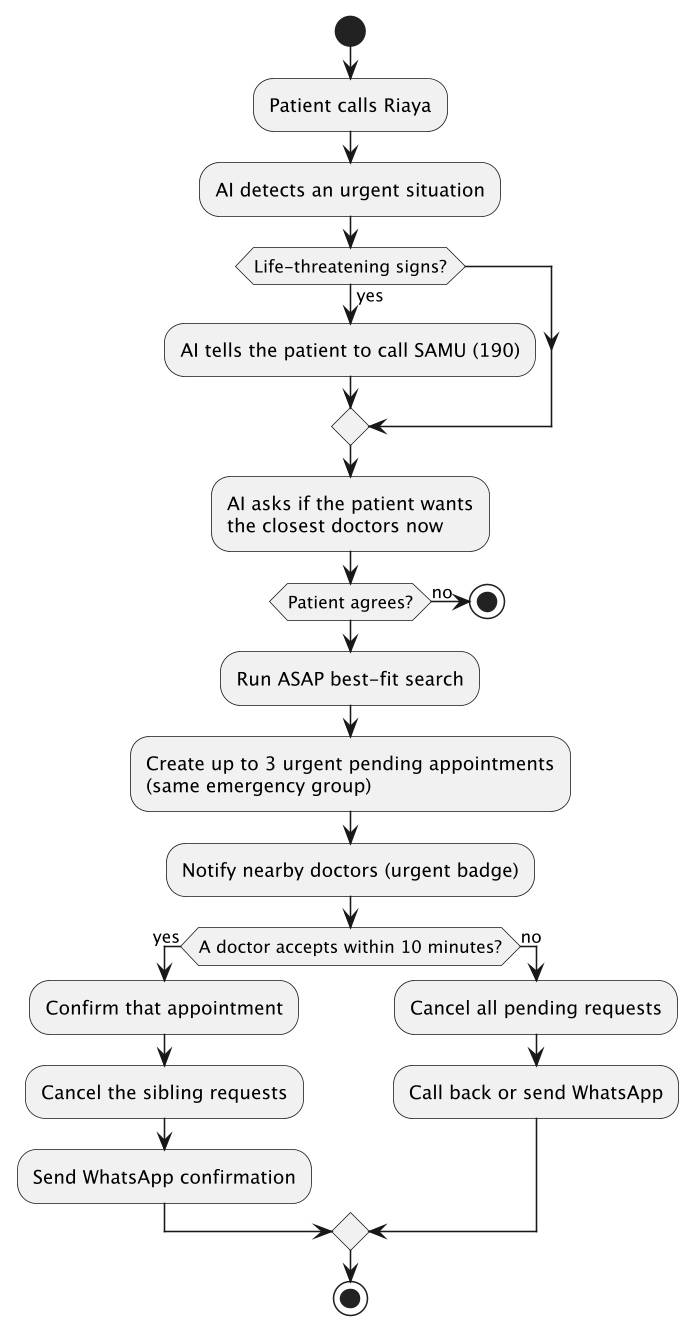
\includegraphics[width=0.8\textwidth]{images/activity_urgent_booking.png}
    \caption{Activity Diagram of the Urgent Booking Process}
    \label{fig:activity_urgent}
\end{figure}

The activity diagram presented in Figure~\ref{fig:activity_urgent} illustrates the workflow of the urgent booking process on the Riaya platform. The flow begins when the patient calls Riaya. The AI assistant detects the urgency of the situation and confirms it with the patient. An ASAP best-fit search is immediately launched, followed by the creation of up to three urgent pending appointments, linked together by an emergency group identifier. Nearby doctors are then notified. A decision point then occurs: if the first doctor accepts within 10 minutes, the appointment is confirmed, the other requests in the group are automatically cancelled, and a confirmation is sent to the patient via WhatsApp. Otherwise, all pending requests are automatically cancelled, and the patient is called back or notified via WhatsApp. The process then ends. This diagram highlights the parallel management of urgent requests and the timeout mechanism that guarantees that no patient is left without a solution.

\begin{figure}[H]
    \centering
    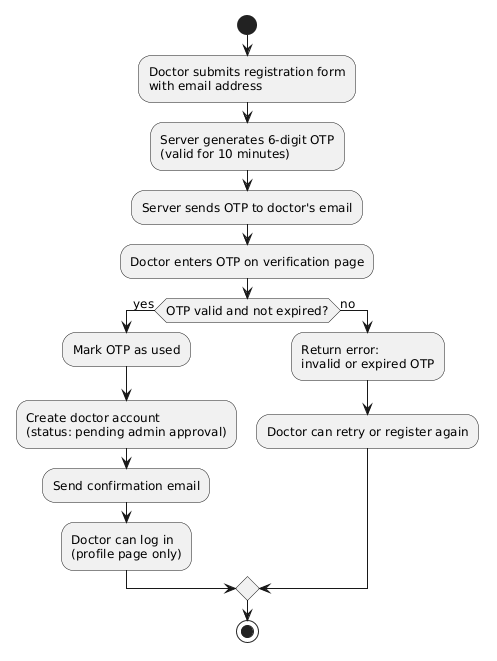
\includegraphics[width=0.8\textwidth]{images/activity_otp_auth.png}
    \caption{Activity Diagram of OTP Authentication}
    \label{fig:activity_otp}
    \small Source: Author's own work based on Riaya internal documentation.
\end{figure}

The activity diagram shown in Figure~\ref{fig:activity_otp} illustrates the OTP-based authentication process used by doctors when registering on the Riaya platform. The process starts when the doctor submits the registration form with an email address. The server then generates a six-digit one-time password (OTP), valid for ten minutes, and sends it to the doctor's email address. The doctor enters the OTP on the verification page. A decision point follows: if the OTP is valid and has not expired, it is marked as used, a doctor account is created with a status of \textit{pending administrator approval}, a confirmation email is sent, and the doctor can log in but can only access the profile page. If the OTP is invalid or expired, an error is returned, and the doctor can either retry entering the OTP or restart the registration process. The process ends after either outcome. This diagram highlights the security measures implemented during registration, including the single-use OTP and the temporary restriction of access until administrator approval.

\subsection{Deployment Diagram: Docker, Nginx, Ubuntu VPS Architecture}
The deployment diagram shows the physical and logical infrastructure of the Riaya platform \cite{docker2024}. It includes:

\begin{itemize}
    \item \textbf{Two repositories:} Web app (Next.js) and Voice server (Express.js). Each repository has its own GitHub Actions CI/CD workflow.
    \item \textbf{GitHub Actions:} CI/CD pipelines that build Docker images, publish them to GHCR, and deploy to a self-hosted Ubuntu VPS.
    \item \textbf{Nginx:} Reverse proxy handling TLS and routing.
    \item \textbf{Docker containers:} PostgreSQL, Redis, web app, and voice server running on a shared Docker network.
    \item \textbf{External services:} Twilio, OpenAI Realtime API (Azure), Cloudflare R2, Konnect.network, WhatsApp Baileys, Geoapify.
\end{itemize}

The deployment diagram also shows the network connections between the different components, including the WebSocket connections between Twilio and the voice server, and between the voice server and the OpenAI Realtime API. It is an essential tool for understanding how the platform is deployed and for planning maintenance and scaling operations.

\begin{figure}[H]
    \centering
    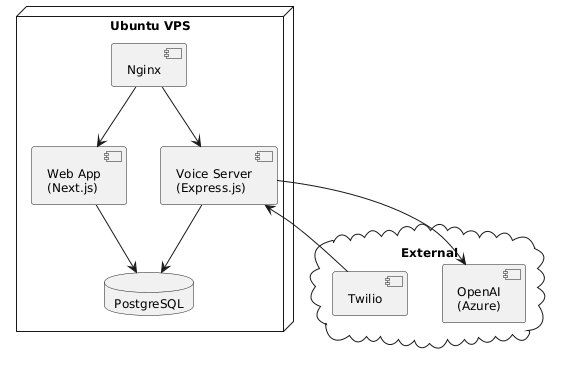
\includegraphics[width=0.9\textwidth]{images/deployment_diagram.png}
    \caption{Deployment Diagram of the Riaya Platform}
    \label{fig:deployment}
\end{figure}

The deployment diagram shown in Figure~\ref{fig:deployment} presents a simplified view of the Riaya platform architecture. The entire system is hosted on an Ubuntu VPS, which runs Nginx as a reverse proxy. Nginx routes HTTP traffic to the Web App (Next.js) and WebSocket connections to the Voice Server (Express.js). Both the Web App and the Voice Server communicate with a PostgreSQL database. The Voice Server also interacts with two external services: it receives incoming phone calls from Twilio and establishes a WebSocket session with the OpenAI Realtime API, which is hosted on Microsoft Azure. This minimal diagram highlights only the core components and their primary connections, omitting secondary services such as Redis, Cloudflare R2, WhatsApp, and payment gateways for clarity.

\subsection{BPMN: Global Business Process}
The BPMN (Business Process Model and Notation) diagram provides a standardized graphical representation of the entire business process of Riaya \cite{omg2011bpmn}. It covers the standard booking flow, the urgent booking flow, and the timeout handling. It includes pools for the patient, the AI system, the doctor, and the administrator, and shows the message flows and sequence flows between them.

The BPMN diagram includes the following main elements:

\begin{itemize}
    \item \textbf{Pools:} Patient, AI System, Doctor, Administrator.
    \item \textbf{Lanes:} Within the AI System pool, lanes for ``Call Handling'', ``Best-fit Search'', ``Appointment Management'', and ``Notification''.
    \item \textbf{Start Events:} Patient calls Riaya, Doctor registers, Administrator logs in.
    \item \textbf{Intermediate Events:} Appointment created, Doctor accepts, Doctor declines, Timeout.
    \item \textbf{End Events:} Appointment confirmed, Appointment cancelled, Registration approved, Registration rejected.
    \item \textbf{Sequence Flows:} The order of activities within each pool.
    \item \textbf{Message Flows:} The communication between pools (e.g., patient calls AI, AI notifies doctor, doctor accepts appointment, AI sends WhatsApp confirmation to patient).
    \item \textbf{Gateways:} Decision points such as ``Is the situation urgent?'' and ``Did the doctor accept within 10 minutes?''.
\end{itemize}

The BPMN diagram is a valuable communication tool that helps both technical and non-technical stakeholders understand the end-to-end process. It also serves as a reference for identifying opportunities for improvement and for ensuring that all scenarios are properly handled.

\begin{figure}[H]
    \centering
    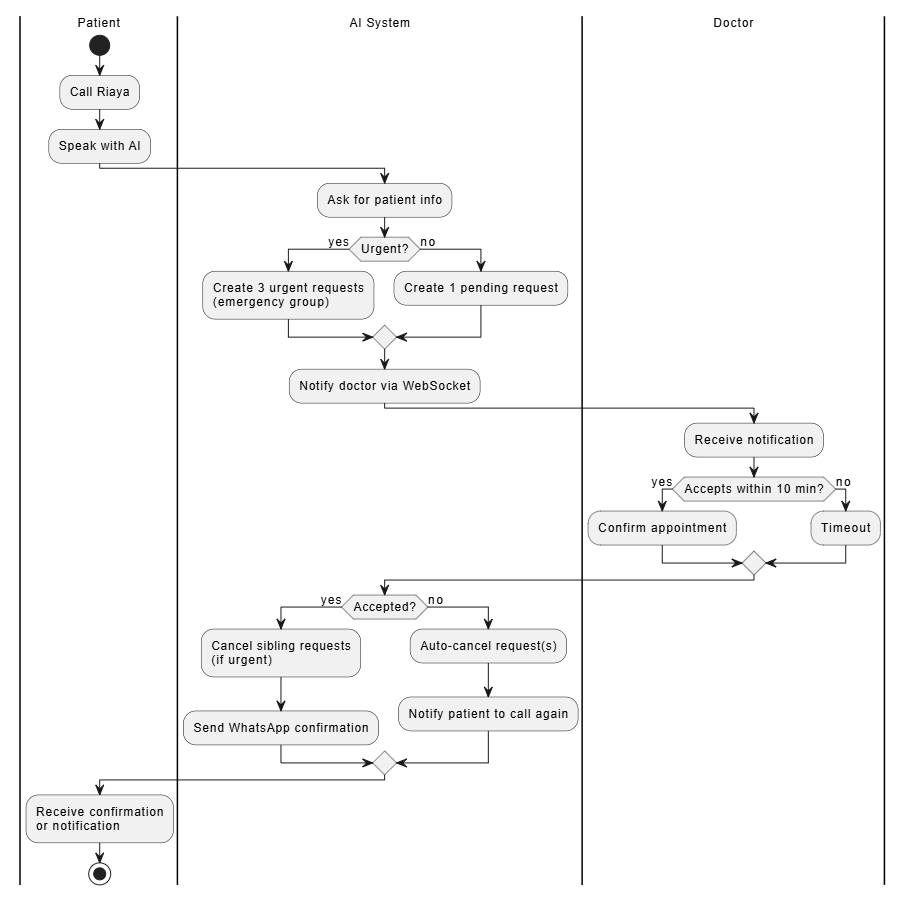
\includegraphics[width=0.9\textwidth]{images/global_bpmn.png}
    \caption{Global BPMN Diagram of the Riaya Project}
    \label{fig:bpmn_global_ch2}
\end{figure}

Figure~\ref{fig:bpmn_global_ch2} presents the global BPMN diagram of the Riaya project, covering all three flows (standard, urgent, and timeout).

\section{Conclusion}
This chapter has presented the Kanban methodology, including its principles, advantages, disadvantages, and a comparative analysis with Scrum and Waterfall. It justified the choice of Kanban for the Riaya project. It also listed and described the main modeling diagrams used in the design of the platform: use case, class/ERD, sequence, activity, deployment, and BPMN. These diagrams provide a solid foundation for understanding both the functional and technical aspects of Riaya. The next chapter will focus on the technical architecture and implementation details.